\documentclass[12pt,halfline,a4paper,]{ouparticle}

% Packages I think are necessary for basic Rmarkdown functionality
\usepackage{hyperref}
\usepackage{graphicx}
\usepackage{listings}
\usepackage{color}
\usepackage{fancyvrb}
\usepackage{framed}

% For knitr::kable functionality
\usepackage{booktabs}
\usepackage{longtable}

%% To allow better options for figure placement
%\usepackage{float}

% Packages that are supposedly required by OUP sty file
\usepackage{amssymb, amsmath, geometry, amsfonts, verbatim, endnotes, setspace}

% For code highlighting I think
\DefineVerbatimEnvironment{Highlighting}{Verbatim}{commandchars=\\\{\}}
\definecolor{shadecolor}{RGB}{248,248,248}
\newenvironment{Shaded}{\begin{snugshade}}{\end{snugshade}}
\newcommand{\AlertTok}[1]{\textcolor[rgb]{0.94,0.16,0.16}{#1}}
\newcommand{\AnnotationTok}[1]{\textcolor[rgb]{0.56,0.35,0.01}{\textbf{\textit{#1}}}}
\newcommand{\AttributeTok}[1]{\textcolor[rgb]{0.77,0.63,0.00}{#1}}
\newcommand{\BaseNTok}[1]{\textcolor[rgb]{0.00,0.00,0.81}{#1}}
\newcommand{\BuiltInTok}[1]{#1}
\newcommand{\CharTok}[1]{\textcolor[rgb]{0.31,0.60,0.02}{#1}}
\newcommand{\CommentTok}[1]{\textcolor[rgb]{0.56,0.35,0.01}{\textit{#1}}}
\newcommand{\CommentVarTok}[1]{\textcolor[rgb]{0.56,0.35,0.01}{\textbf{\textit{#1}}}}
\newcommand{\ConstantTok}[1]{\textcolor[rgb]{0.00,0.00,0.00}{#1}}
\newcommand{\ControlFlowTok}[1]{\textcolor[rgb]{0.13,0.29,0.53}{\textbf{#1}}}
\newcommand{\DataTypeTok}[1]{\textcolor[rgb]{0.13,0.29,0.53}{#1}}
\newcommand{\DecValTok}[1]{\textcolor[rgb]{0.00,0.00,0.81}{#1}}
\newcommand{\DocumentationTok}[1]{\textcolor[rgb]{0.56,0.35,0.01}{\textbf{\textit{#1}}}}
\newcommand{\ErrorTok}[1]{\textcolor[rgb]{0.64,0.00,0.00}{\textbf{#1}}}
\newcommand{\ExtensionTok}[1]{#1}
\newcommand{\FloatTok}[1]{\textcolor[rgb]{0.00,0.00,0.81}{#1}}
\newcommand{\FunctionTok}[1]{\textcolor[rgb]{0.00,0.00,0.00}{#1}}
\newcommand{\ImportTok}[1]{#1}
\newcommand{\InformationTok}[1]{\textcolor[rgb]{0.56,0.35,0.01}{\textbf{\textit{#1}}}}
\newcommand{\KeywordTok}[1]{\textcolor[rgb]{0.13,0.29,0.53}{\textbf{#1}}}
\newcommand{\NormalTok}[1]{#1}
\newcommand{\OperatorTok}[1]{\textcolor[rgb]{0.81,0.36,0.00}{\textbf{#1}}}
\newcommand{\OtherTok}[1]{\textcolor[rgb]{0.56,0.35,0.01}{#1}}
\newcommand{\PreprocessorTok}[1]{\textcolor[rgb]{0.56,0.35,0.01}{\textit{#1}}}
\newcommand{\RegionMarkerTok}[1]{#1}
\newcommand{\SpecialCharTok}[1]{\textcolor[rgb]{0.00,0.00,0.00}{#1}}
\newcommand{\SpecialStringTok}[1]{\textcolor[rgb]{0.31,0.60,0.02}{#1}}
\newcommand{\StringTok}[1]{\textcolor[rgb]{0.31,0.60,0.02}{#1}}
\newcommand{\VariableTok}[1]{\textcolor[rgb]{0.00,0.00,0.00}{#1}}
\newcommand{\VerbatimStringTok}[1]{\textcolor[rgb]{0.31,0.60,0.02}{#1}}
\newcommand{\WarningTok}[1]{\textcolor[rgb]{0.56,0.35,0.01}{\textbf{\textit{#1}}}}

% For making Rmarkdown lists
\providecommand{\tightlist}{%
  \setlength{\itemsep}{0pt}\setlength{\parskip}{0pt}}

% Part for setting citation format package: natbib

% Part for setting citation format package: biblatex

% Part for indenting CSL refs

% Pandoc header

\begin{document}

\title{Final Exam Practice}

\author{%
\name{YOUR NAME HERE}\address{University of Georgia}\email{\href{mailto:email@email.email}{email@email.email}}
\and
\name{Joseph T. Ornstein}\address{University of Georgia}\email{\href{mailto:jornstein@uga.edu}{jornstein@uga.edu}}
}

\abstract{}

\date{December 04, 2020}

\keywords{}

\maketitle



\hypertarget{introduction}{%
\section{Introduction}\label{introduction}}

In this paper, we will replicate the results from ``Civic Honesty Around
the Globe'' (Cohn et al. 2019). Anything I call an ``extra challenge''
is available for the intrepid among you, but is not required.

To submit your final exam, knit this \texttt{.Rmd} to a PDF and post it
to eLC.

\hypertarget{data}{%
\section{Data}\label{data}}

Replication files are available
\href{https://dataverse.harvard.edu/dataverse/honesty}{here}, and I have
already downloaded them into the \texttt{data/} folder. Let's load the
behavioral data.

\begin{Shaded}
\begin{Highlighting}[]
\NormalTok{data <-}\StringTok{ }\KeywordTok{read_csv}\NormalTok{(}\StringTok{'data/behavioral data (csv file).csv'}\NormalTok{)}
\end{Highlighting}
\end{Shaded}

\hypertarget{results}{%
\section{Results}\label{results}}

\hypertarget{replicating-figure-1}{%
\subsection{Replicating Figure 1}\label{replicating-figure-1}}

First, let's replicate the left-hand side of Figure 1. To do so, we need
to perform the following steps:

\begin{itemize}
\tightlist
\item
  Keep only the \texttt{Money} and \texttt{NoMoney} conditions.
\item
  Recode the \texttt{cond} variable as ``Money'' and ``NoMoney''.
\item
  Compute the average response rate, grouped by country and condition.
\item
  Plot a scatter with reporting rate on the x-axis, country on the
  y-axis, and colored by monetary condition.
\end{itemize}

As an extra challenge, you can:

\begin{itemize}
\tightlist
\item
  Rearrange the y-axis so that the countries with the lowest reporting
  rate appear at the bottom and those with the highest reporting rate
  appear at the top.
\item
  Include the line segments between points from the original figure
\item
  Use the colors from the original figure
\end{itemize}

\begin{Shaded}
\begin{Highlighting}[]
\NormalTok{fig1 <-}\StringTok{ }\NormalTok{data }\OperatorTok\StringTok{ }
\StringTok{  }\KeywordTok{filter}\NormalTok{(cond }\OperatorTok\StringTok{ }\KeywordTok{c}\NormalTok{(}\DecValTok{0}\NormalTok{,}\DecValTok{1}\NormalTok{)) }\OperatorTok\StringTok{ }
\StringTok{  }\KeywordTok{mutate}\NormalTok{(}\DataTypeTok{cond =} \KeywordTok{case_when}\NormalTok{(cond }\OperatorTok{==}\StringTok{ }\DecValTok{1} \OperatorTok{~}\StringTok{ 'Money'}\NormalTok{, }
\NormalTok{                          cond }\OperatorTok{==}\StringTok{ }\DecValTok{0} \OperatorTok{~}\StringTok{ 'NoMoney'}\NormalTok{)) }\OperatorTok\StringTok{ }
\StringTok{  }\CommentTok{# compute reporting rate by country and monetary condition}
\StringTok{  }\KeywordTok{group_by}\NormalTok{(Country,}
\NormalTok{           cond) }\OperatorTok\StringTok{ }
\StringTok{  }\KeywordTok{summarize}\NormalTok{(}\DataTypeTok{pct_reported =} \KeywordTok{mean}\NormalTok{(response)) }\OperatorTok
\StringTok{  }\CommentTok{# # sort by reporting rate}
\StringTok{  }\CommentTok{# ungroup %>% }
\StringTok{  }\CommentTok{# arrange(pct_reported) %>% }
\StringTok{  }\CommentTok{# mutate(Country = factor(Country, levels = unique(Country))) %>% }
\StringTok{  }\CommentTok{# plot}
\StringTok{  }\KeywordTok{ggplot}\NormalTok{() }\OperatorTok{+}
\StringTok{  }\KeywordTok{geom_point}\NormalTok{(}\KeywordTok{aes}\NormalTok{(}\DataTypeTok{x=}\NormalTok{pct_reported, }\DataTypeTok{y=}\NormalTok{Country, }\DataTypeTok{color =} \KeywordTok{factor}\NormalTok{(cond))) }\OperatorTok{+}
\StringTok{  }\KeywordTok{labs}\NormalTok{(}\DataTypeTok{x =} \StringTok{'Reporting rate (%)'}\NormalTok{, }\DataTypeTok{y =} \StringTok{''}\NormalTok{, }\DataTypeTok{color =} \StringTok{'Condition'}\NormalTok{) }\OperatorTok{+}
\StringTok{  }\KeywordTok{theme_minimal}\NormalTok{()}

\NormalTok{fig1}
\end{Highlighting}
\end{Shaded}

\begin{figure}[p]
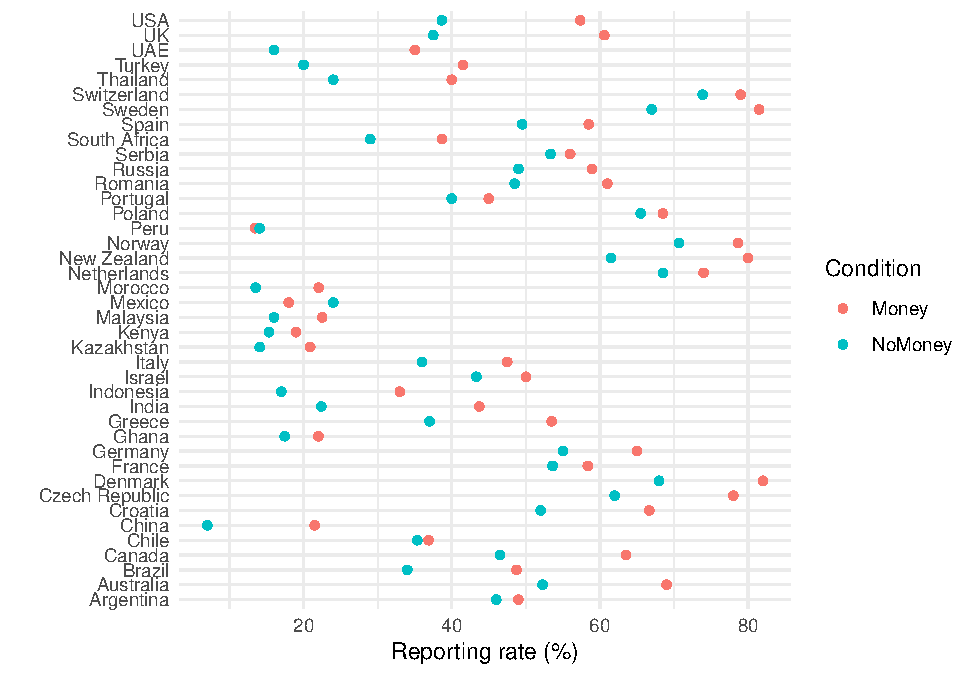
\includegraphics[width=1\linewidth]{Civic-Honesty-Replication_files/figure-latex/Figure 1-1} \caption{Share of wallets reported in the NoMoney and Money conditions, by country.}\label{fig:Figure 1-1}
\end{figure}

\begin{Shaded}
\begin{Highlighting}[]
\CommentTok{# Here's the challenging one}
\NormalTok{fig1a <-}\StringTok{ }\NormalTok{data }\OperatorTok\StringTok{ }
\StringTok{  }\KeywordTok{filter}\NormalTok{(cond }\OperatorTok\StringTok{ }\KeywordTok{c}\NormalTok{(}\DecValTok{0}\NormalTok{,}\DecValTok{1}\NormalTok{)) }\OperatorTok\StringTok{ }
\StringTok{  }\KeywordTok{mutate}\NormalTok{(}\DataTypeTok{cond =} \KeywordTok{case_when}\NormalTok{(cond }\OperatorTok{==}\StringTok{ }\DecValTok{1} \OperatorTok{~}\StringTok{ 'Money'}\NormalTok{, }
\NormalTok{                          cond }\OperatorTok{==}\StringTok{ }\DecValTok{0} \OperatorTok{~}\StringTok{ 'NoMoney'}\NormalTok{)) }\OperatorTok\StringTok{ }
\StringTok{  }\CommentTok{# compute reporting rate by country and monetary condition}
\StringTok{  }\KeywordTok{group_by}\NormalTok{(Country,}
\NormalTok{           cond) }\OperatorTok\StringTok{ }
\StringTok{  }\KeywordTok{summarize}\NormalTok{(}\DataTypeTok{pct_reported =} \KeywordTok{mean}\NormalTok{(response)) }\OperatorTok
\StringTok{  }\CommentTok{# pivot_wider to make those line segments}
\StringTok{  }\NormalTok{ungroup }\OperatorTok\StringTok{ }
\StringTok{  }\KeywordTok{pivot_wider}\NormalTok{(}\DataTypeTok{names_from =}\NormalTok{ cond, }\DataTypeTok{values_from =}\NormalTok{ pct_reported) }\OperatorTok\StringTok{ }
\StringTok{  }\CommentTok{# sort by NoMoney reporting rate}
\StringTok{  }\KeywordTok{arrange}\NormalTok{(NoMoney) }\OperatorTok\StringTok{ }
\StringTok{  }\KeywordTok{mutate}\NormalTok{(}\DataTypeTok{Country =} \KeywordTok{factor}\NormalTok{(Country, }\DataTypeTok{levels =} \KeywordTok{unique}\NormalTok{(Country))) }\OperatorTok\StringTok{ }
\StringTok{  }\KeywordTok{ggplot}\NormalTok{() }\OperatorTok{+}
\StringTok{  }\KeywordTok{geom_segment}\NormalTok{(}\KeywordTok{aes}\NormalTok{(}\DataTypeTok{x=}\NormalTok{Money, }\DataTypeTok{xend=}\NormalTok{NoMoney, }\DataTypeTok{y=}\NormalTok{Country, }\DataTypeTok{yend=}\NormalTok{Country),}
               \DataTypeTok{color =} \StringTok{'gray'}\NormalTok{, }\DataTypeTok{size =} \FloatTok{0.5}\NormalTok{) }\OperatorTok{+}\StringTok{ }
\StringTok{  }\KeywordTok{geom_point}\NormalTok{(}\KeywordTok{aes}\NormalTok{(}\DataTypeTok{x=}\NormalTok{Money,}\DataTypeTok{y=}\NormalTok{Country), }\DataTypeTok{color =} \StringTok{'red'}\NormalTok{) }\OperatorTok{+}
\StringTok{  }\KeywordTok{geom_point}\NormalTok{(}\KeywordTok{aes}\NormalTok{(}\DataTypeTok{x=}\NormalTok{NoMoney,}\DataTypeTok{y=}\NormalTok{Country), }\DataTypeTok{color =} \StringTok{'#F6BE00'}\NormalTok{) }\OperatorTok{+}
\StringTok{  }\KeywordTok{geom_text}\NormalTok{(}\KeywordTok{aes}\NormalTok{(}\DataTypeTok{x=}\NormalTok{NoMoney}\DecValTok{-3}\NormalTok{, }\DataTypeTok{y=}\NormalTok{Country, }\DataTypeTok{label =}\NormalTok{ Country), }\DataTypeTok{size =} \DecValTok{2}\NormalTok{) }\OperatorTok{+}
\StringTok{  }\KeywordTok{labs}\NormalTok{(}\DataTypeTok{x =} \StringTok{'Reporting rate (%)'}\NormalTok{, }\DataTypeTok{y =} \StringTok{''}\NormalTok{, }\DataTypeTok{color =} \StringTok{'Condition'}\NormalTok{) }\OperatorTok{+}
\StringTok{  }\KeywordTok{theme_classic}\NormalTok{() }\OperatorTok{+}
\StringTok{  }\KeywordTok{theme}\NormalTok{(}\DataTypeTok{axis.text.y =} \KeywordTok{element_blank}\NormalTok{(),}
        \DataTypeTok{axis.ticks.y =} \KeywordTok{element_blank}\NormalTok{())}
  
  

\NormalTok{fig1a}
\end{Highlighting}
\end{Shaded}

\begin{figure}[p]
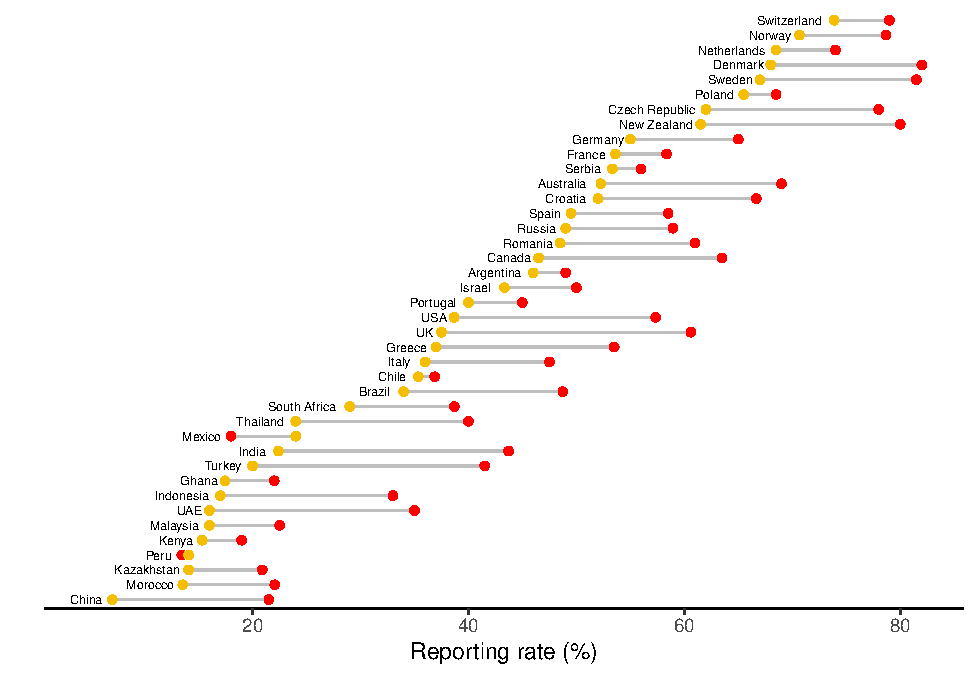
\includegraphics[width=1\linewidth]{Civic-Honesty-Replication_files/figure-latex/Figure 1-2} \caption{Share of wallets reported in the NoMoney and Money conditions, by country.}\label{fig:Figure 1-2}
\end{figure}

\hypertarget{references}{%
\section*{References}\label{references}}
\addcontentsline{toc}{section}{References}

\hypertarget{refs}{}
\leavevmode\hypertarget{ref-cohnCivicHonestyGlobe2019}{}%
Cohn, Alain, Michel André Maréchal, David Tannenbaum, and Christian
Lukas Zünd. 2019. ``Civic Honesty Around the Globe.'' \emph{Science} 365
(6448): 70--73. \url{https://doi.org/10.1126/science.aau8712}.






\end{document}
